\documentclass{style/CRPITStyle}
\usepackage{epsfig}   % Packages to use if you wish
\usepackage{lscape}   %
\usepackage[authoryear]{natbib}
\renewcommand{\cite}{\citep}
\pagestyle{empty}
\thispagestyle{empty}
\hyphenation{roddick}

\begin{document}

\title{Software Development: An Evaluation of KPSmart Development}
\author{David Barnett}
\affiliation{School of Engineering and Computer Science \\
Victoria University of Wellington, \\
PO Box 600, Wellington, 6140 \\
Email:~{\tt barentdavi@myvuw.ac.nz}}

\maketitle

\begin{abstract}
\end{abstract}

\vspace{.1in}

\noindent {\em Keywords:}\/ System, Iterative and Incremental Development, Group Project

\vspace{.1in}

\section{Introduction}

% Which process model your team has chosen for the project and why, and
% how your team used the process model,
\section{Process Model}

\begin{figure}[htb]
\fbox{\parbox[b]{.99\linewidth}{
\vskip 0.5cm
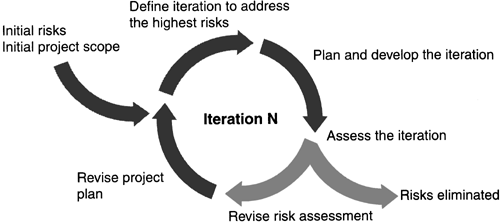
\includegraphics[width=0.45\textwidth]{figures/iid-model.png}
\vskip 0.5cm}}
\caption{\protect\label{s-system} Incremental and Iterative development model }
\end{figure}

%The experiences you made with using the process model and the lessons
% you learned from the project
\section{Experience}
% andrew: pretty kewl
% cuan: late?
% Cameron price:
% Cameron Porter:
% me:


% How well your application meets the requirements gathered during the
% initial requirements analysis and what you have done to ensure your ap-
% plication meets the requirements
\section{Requirements}

% What kind of system is your application, i.e., S-system, E-system or P-
% system and why?
\section{System Type}
% Define, what the 3 system types are
% point out which parts of the system display symptoms of that system
% and which points it misses
% big reveal it is P-System!!!

A software program can be described as one of three types of systems:
S-System, E-System and P-System. Each type of system has a varying set of traits
to their development and maintenance cycles as they have different relationships
to their environments and specifications that they were designed for and how
they react to changes in either of them. These range from development
and maintenance is continuous to after development there is no need for
maintenance. The KPSmart application displays some traits of each of system
types but mostly exhibits the traits of a P-System.

\subsection{S-System}

The KPSmart application has some traits of a S-System. Which are broadly described as
systems which has its functionality formally defined by the specification as
well as how it will be delivered \cite{lehman:1980}.
This focus on specification is what puts the \emph{S} into \emph{S}-System.
In practice S-Systems are systems which
solve a problem which is related to the real world with very rigid rules such
as implementing a sorting algorithm which leads onto a set of well defined
specifications for the system to be implemented.
Changing the specifications, and thus the problem the system is to solve,
would results in changing the system as a whole due to the system being tightly
coupled. The maintenance of a S-System would be low as the resulting system
would not need to change unless its specifications does.
This process is illustrated by the figure \ref{s-system}.

\vspace{.1in}

\begin{figure}[htb]
\fbox{\parbox[b]{.99\linewidth}{
\vskip 0.5cm
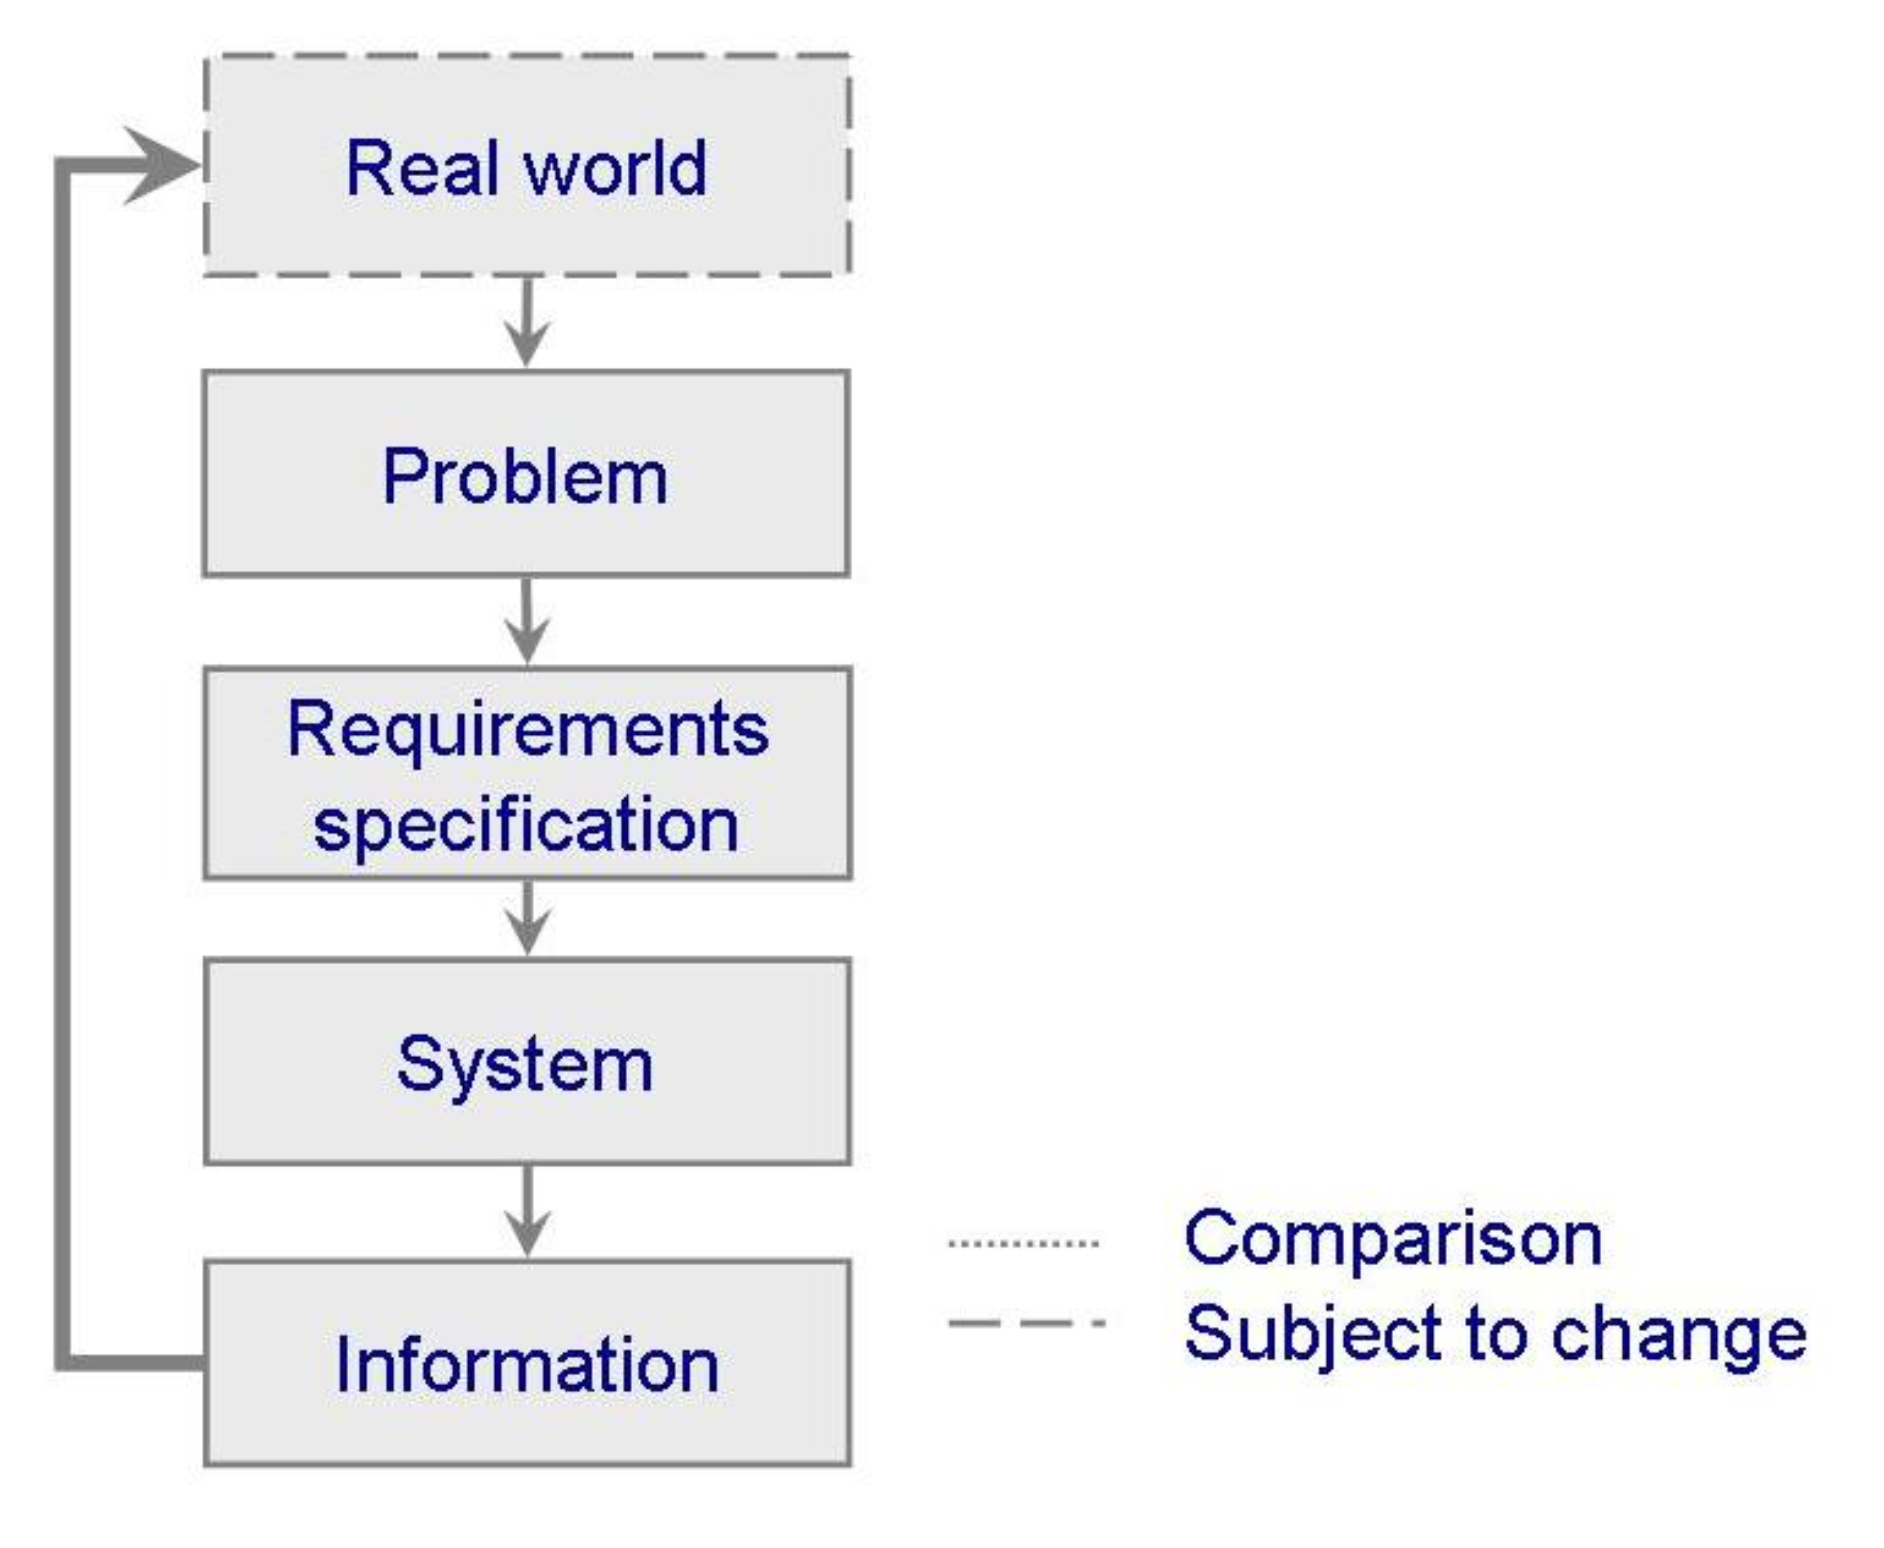
\includegraphics[width=0.45\textwidth]{figures/s-system.png}
\vskip 0.5cm}}
\caption{\protect\label{s-system} S-System}
\end{figure}

\vspace{.1in}

The KPSmart application itself is formally defined by specifications to solve a
problem but lacks the level of details and rigidity to classify it as an
S-System, however some sub-systems of the applications are fit to be classed as such.
These include the routing and the calculation for a mail delivery duration
sub-systems as they both are well defined in what problem they solve.

\subsection{E-System}

The KPS application has some aspects of an E-System.
An E-System is

\vspace{.1in}

\begin{figure}[htb]
\fbox{\parbox[b]{.99\linewidth}{
\vskip 0.5cm
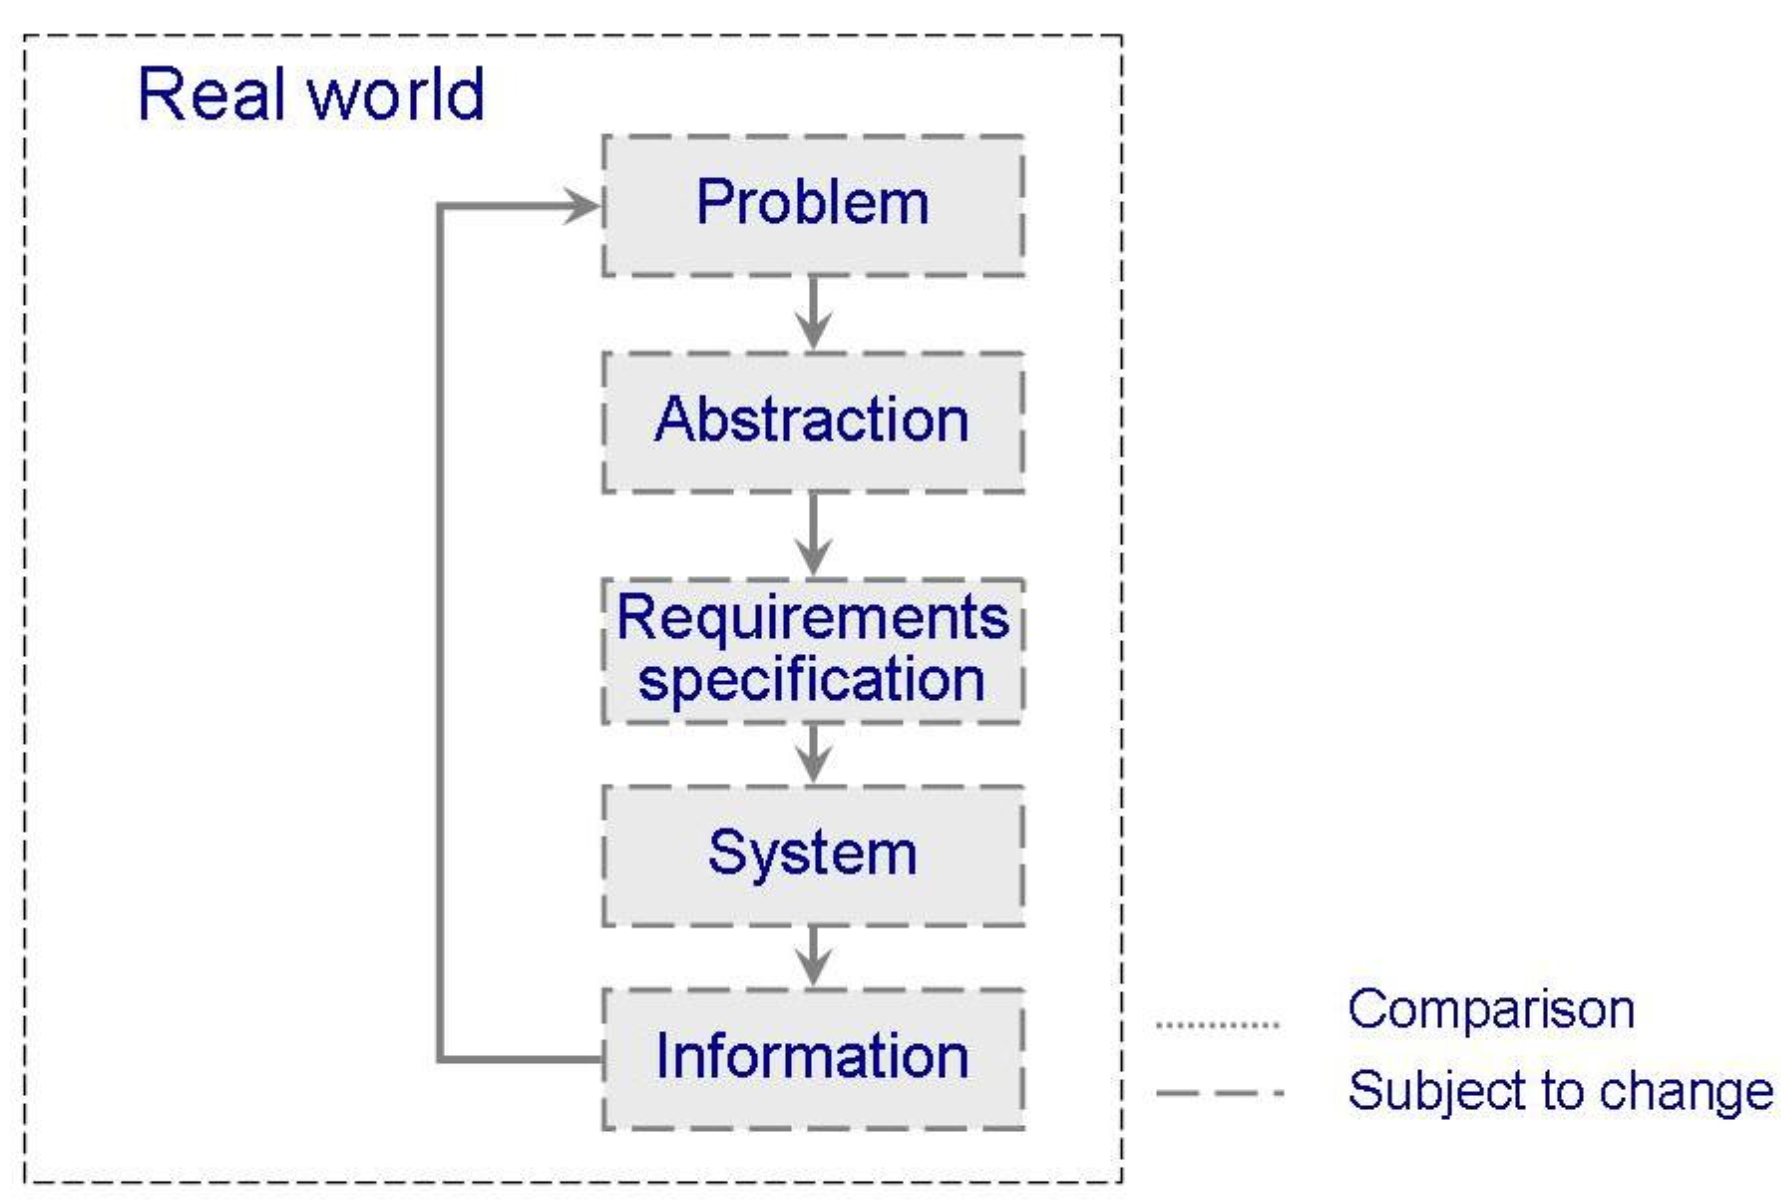
\includegraphics[width=0.45\textwidth]{figures/e-system.png}
\vskip 0.5cm}}
\caption{\protect\label{e-system}  E-System }
\end{figure}

\vspace{.1in}

\subsection{P-System}

\vspace{.1in}

\begin{figure}[htb]
\fbox{\parbox[b]{.99\linewidth}{
\vskip 0.5cm
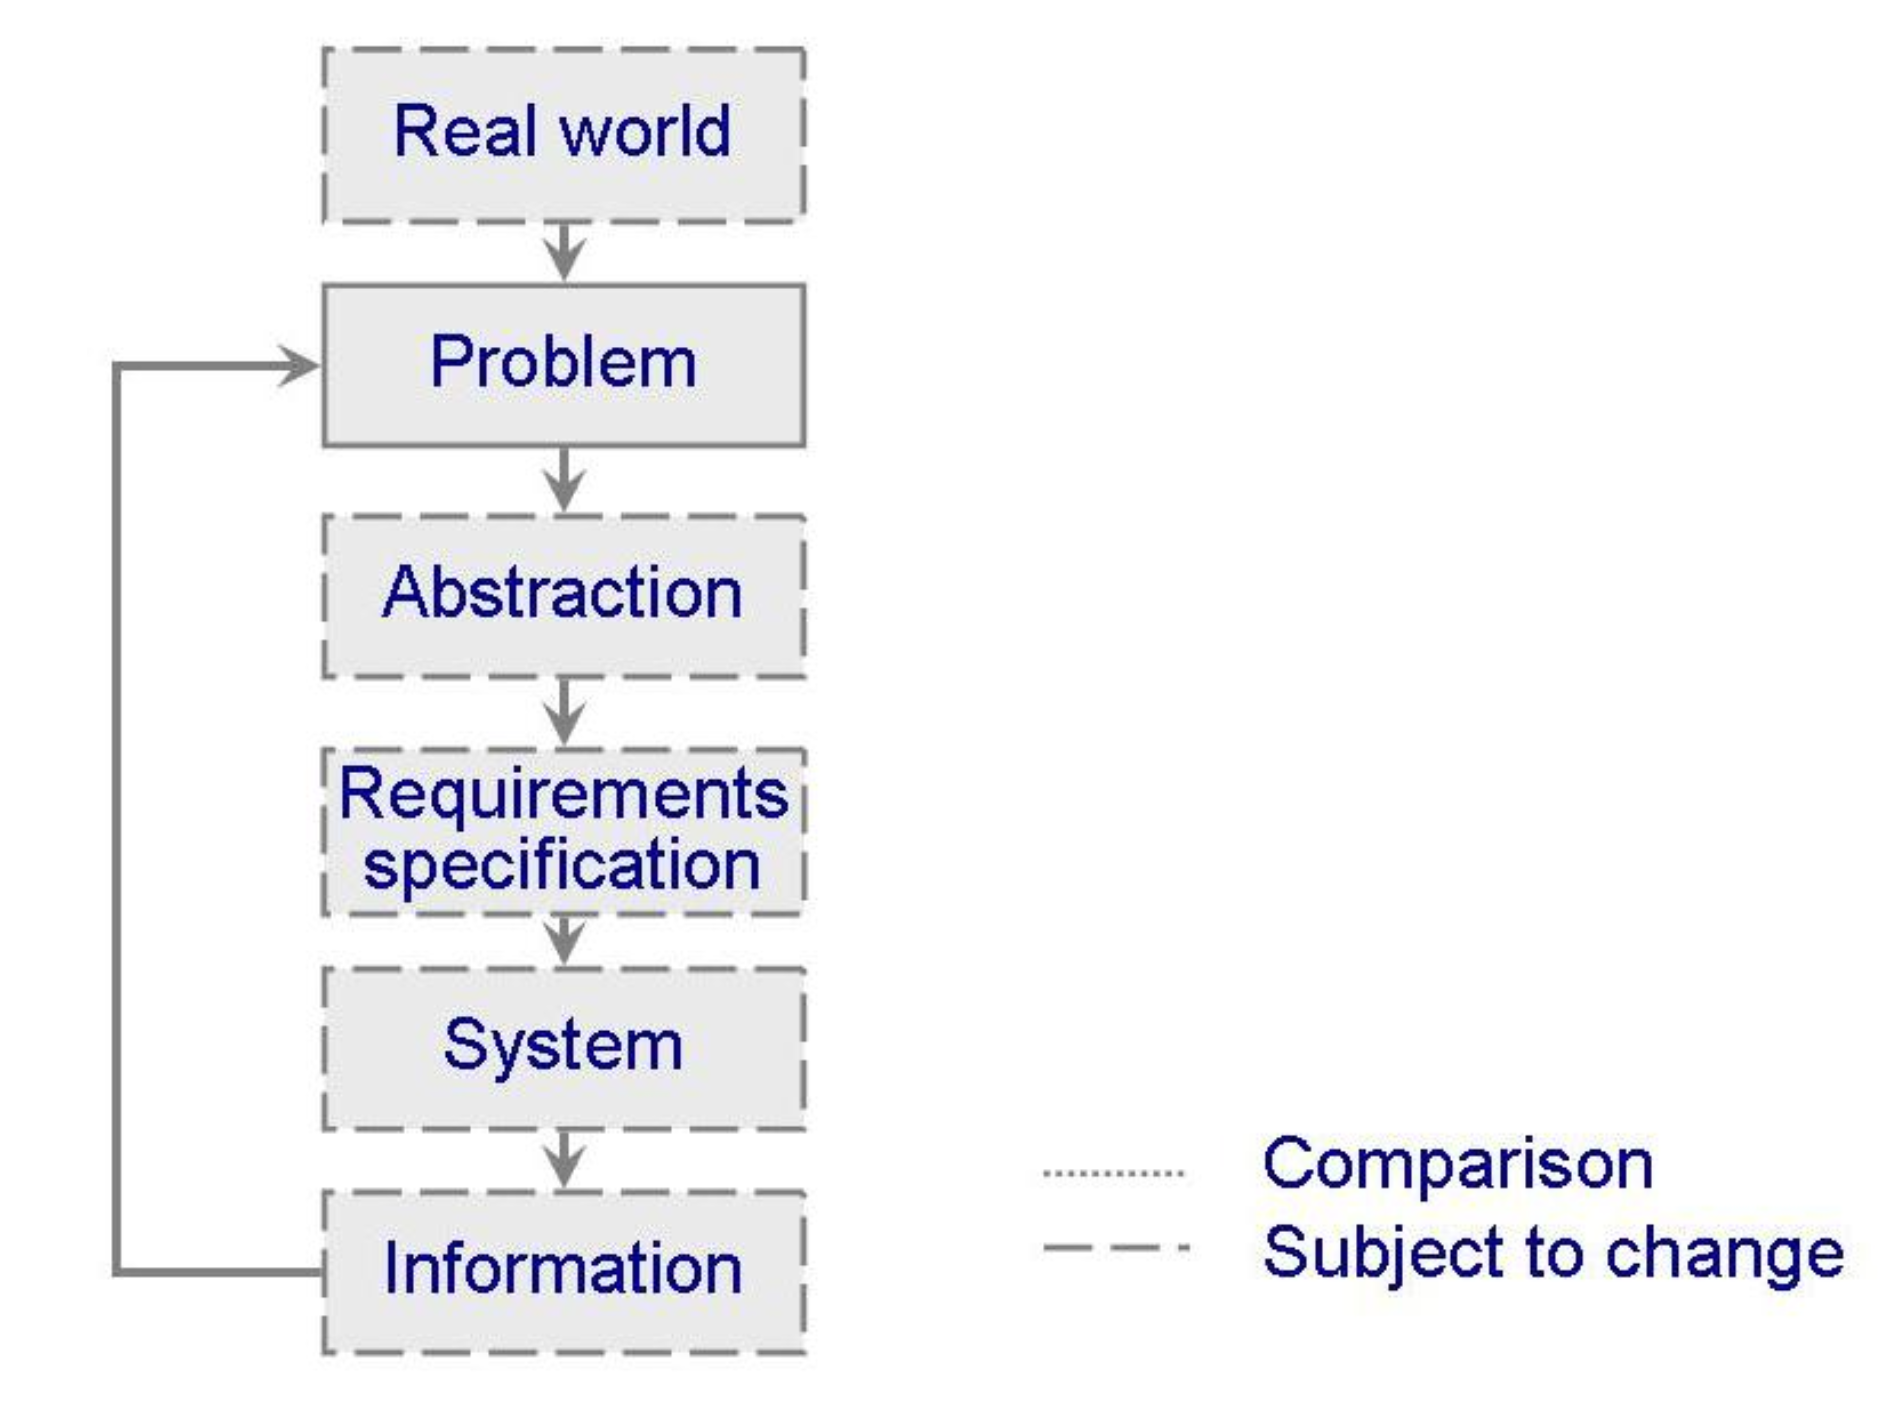
\includegraphics[width=0.45\textwidth]{figures/p-system.png}
\vskip 0.5cm}}
\caption{\protect\label{p-system}  P-System }
\end{figure}

\vspace{.1in}

% What kind of maintenance activities may be needed to maintain the ap-
% plication. Recall that four types of software maintenance activities were
% discussed in the lectures.
\section{Maintenance}

% What process model would you use if the project were developed as an
% open source application, and why?  Which Indirect Sale-Value model,
% discussed in the lecture, can be used for your application, and how?
\section{Open source}

\cite{raymond:1999}

\section{Conclusion}

\bibliographystyle{agsm}
\bibliography{report}

\end{document}

% vim:set spell et sw=4 ts=4 tw=80:
